\section{Basic System Design}
\label{sec:system-design}

We use the same system design presented by PacketShader and Gnort. Pictured in
Figure~\ref{fig:system}, packets pass through our system as follows: (1) As
packets arrive at the NIC, they are copied to main memory via DMA. (2) Software
running on the CPU copies these new packets to a buffer until a sufficient
number have arrived (see below) and (3) the batch is transferred to memory on
the GPU. (4) The GPU processes the packets in parallel and fills a buffer of
results on the GPU which (5) the CPU copies back to main memory when processing
has finished. (6) Using these results, the CPU instructs the NIC(s) where to
forward each packet in the batch; (7) finally, the NIC(s) fetch(es) the packets
from main memory with another DMA and forwards them.

\begin{figure}
   \centering
   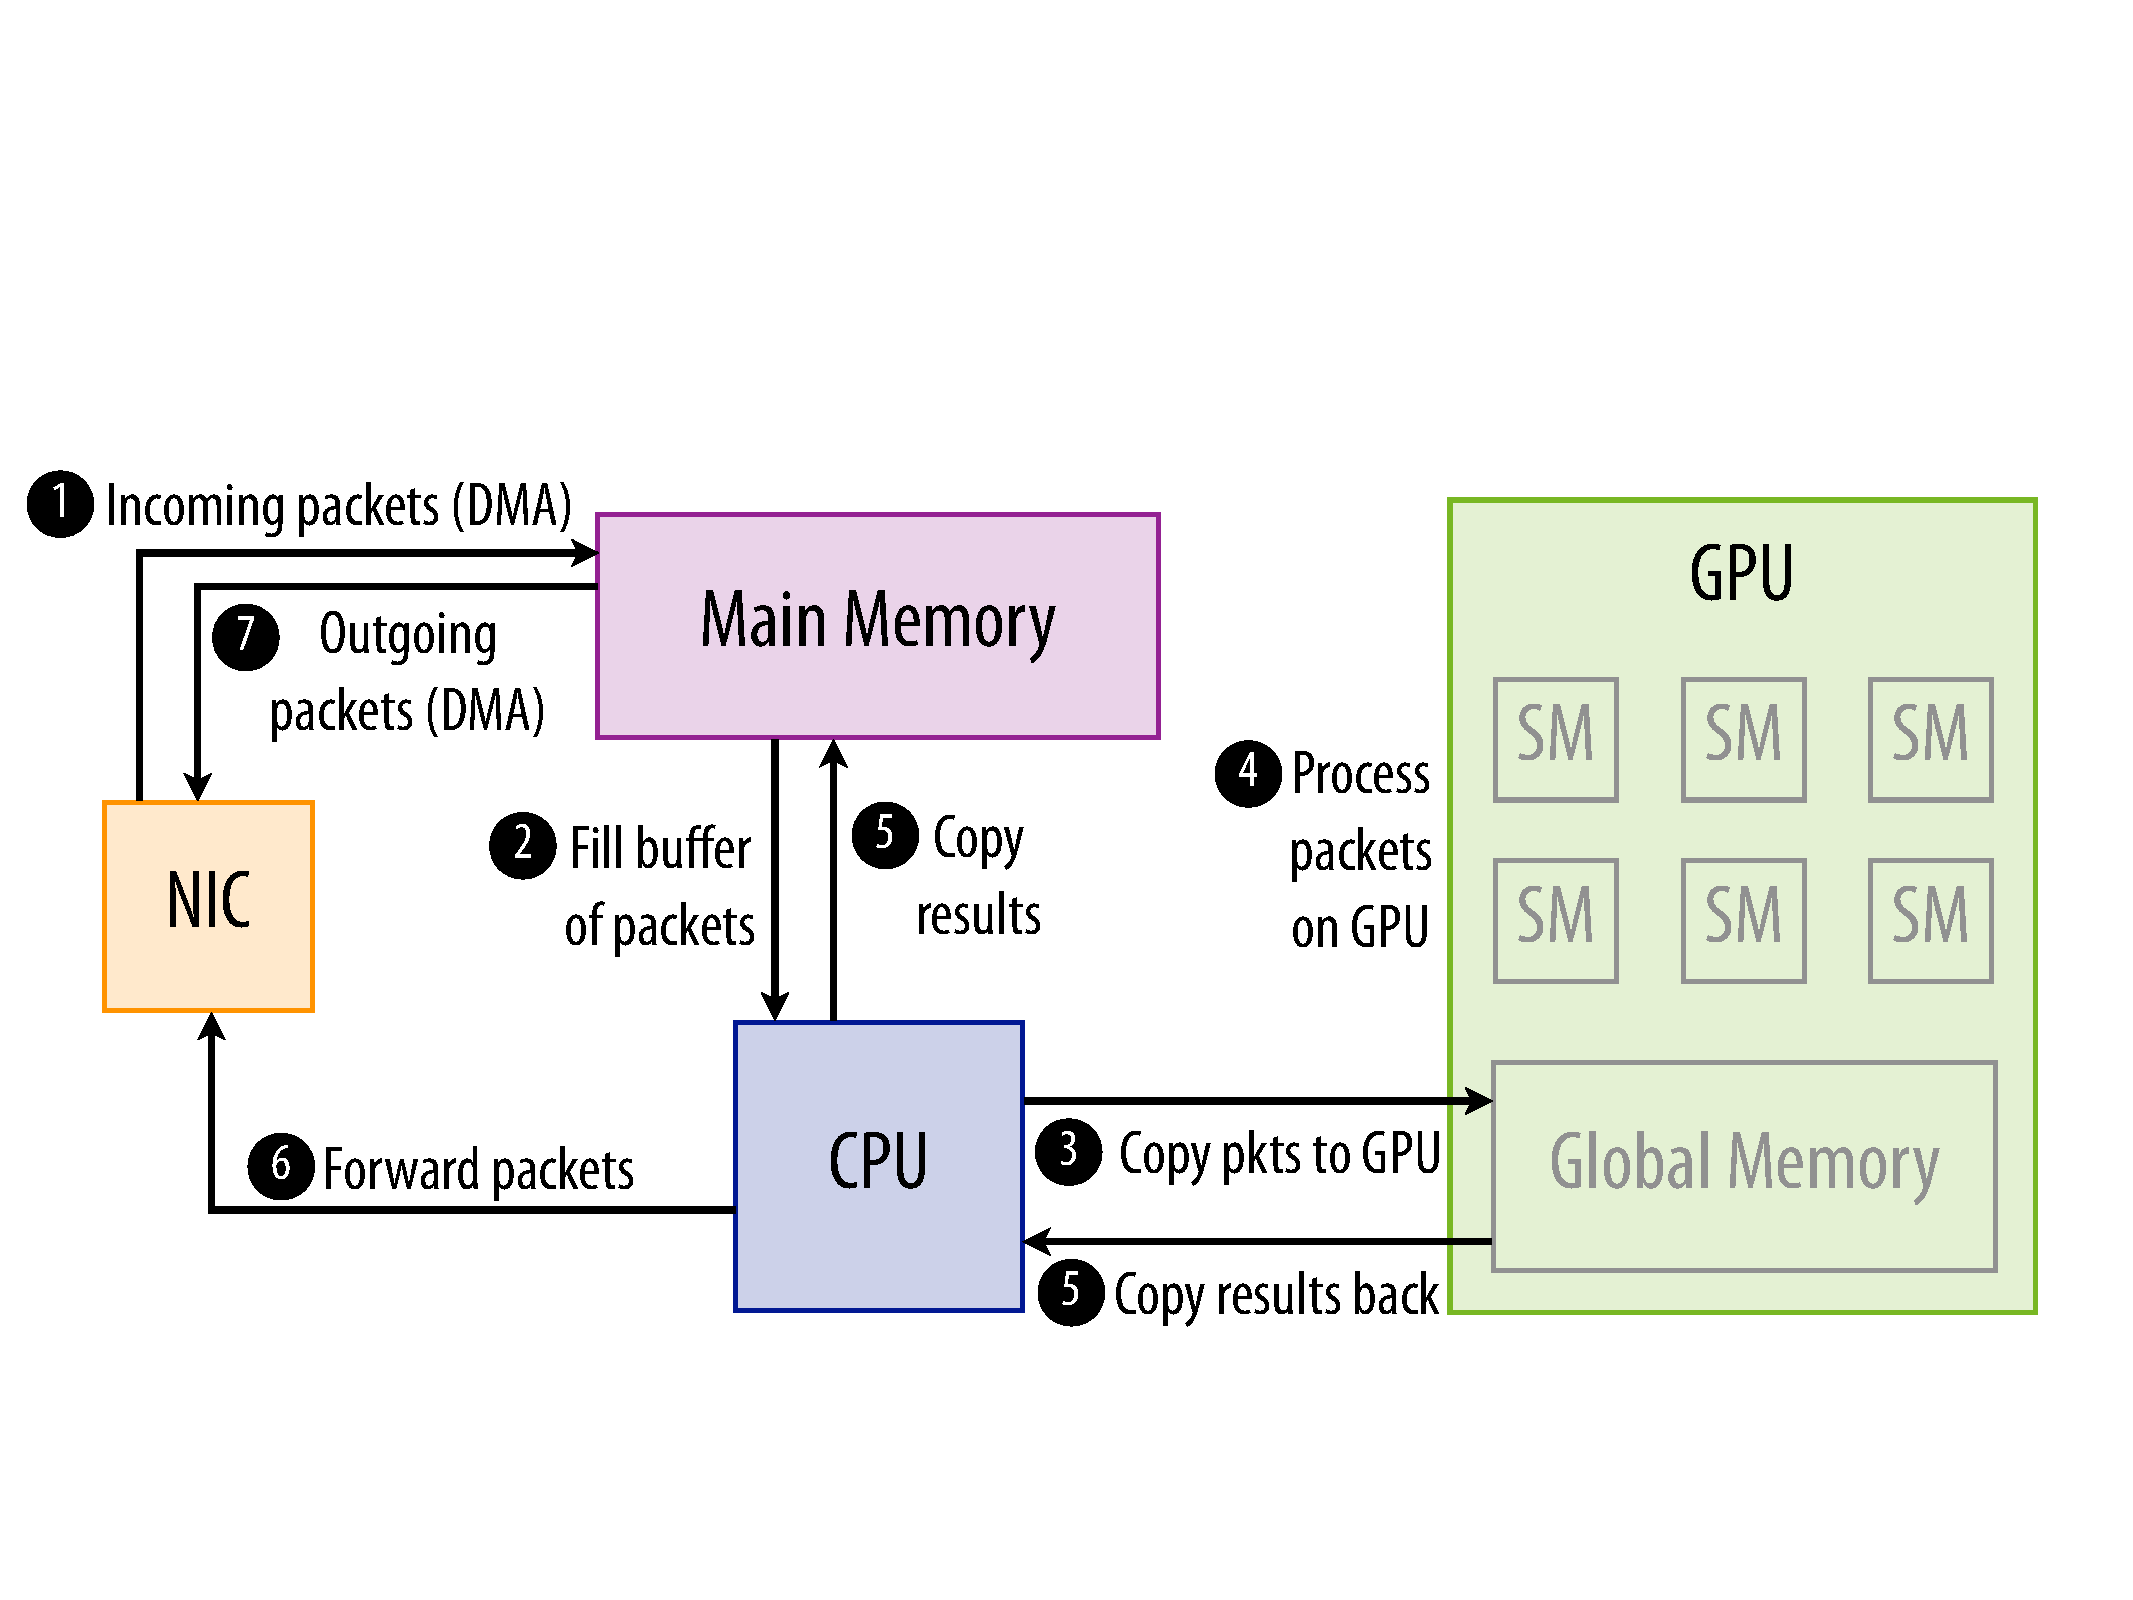
\includegraphics[scale=0.23]{figs/system_overview.pdf} 
   \caption{Basic System Design}
   \label{fig:system}
\end{figure}

\subsection{GPU Programming Issues}
\noindent \textbf{Pipelining.} As with almost any CUDA program, ours employs
pipelining for data transfers between main memory and GPU memory. While the GPU
is busy processing a batch of packets, we can utilize the CPU to copy the
results from the previous batch of packets from the GPU back to main memory and
copy the next batch of packets to the GPU (Figure~\ref{fig:pipelining}). In
this way, we never let CPU cycles go idle while the GPU is working.\\

\begin{figure}
   \centering
   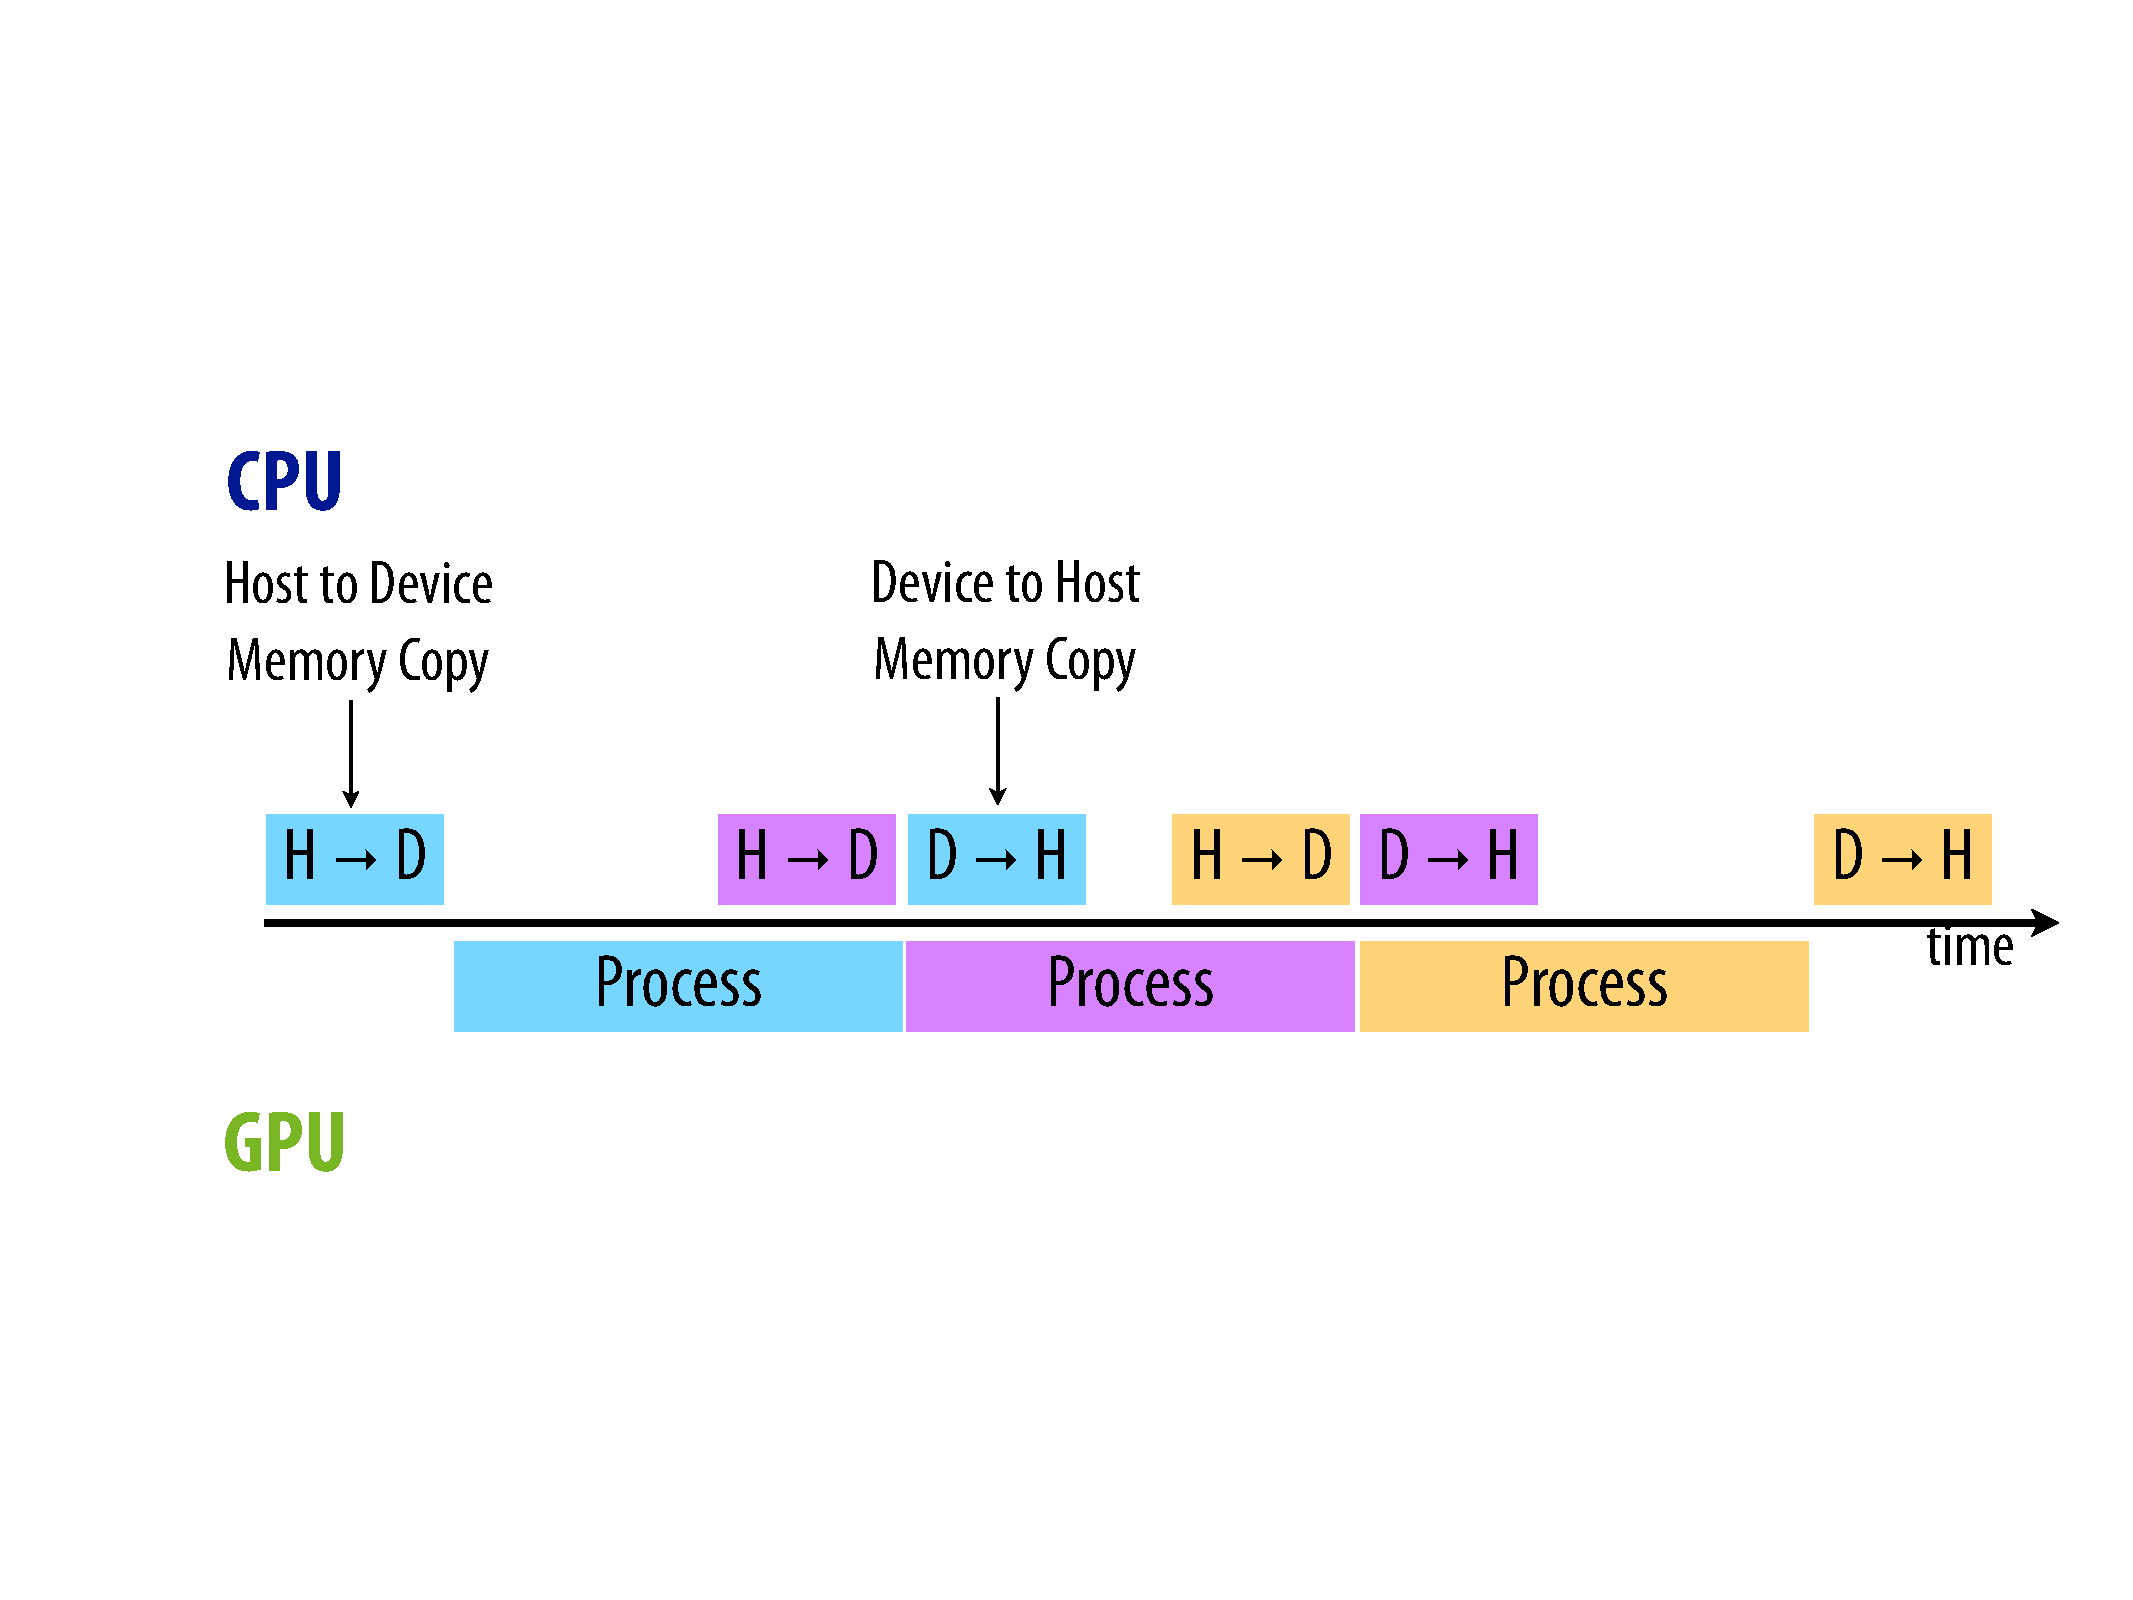
\includegraphics[scale=0.25]{figs/pipelining.pdf}
   \caption{Pipelined Execution}
   \label{fig:pipelining}
\end{figure}

\medskip \noindent \textbf{Batching.} Although the GPU can process hundreds of
packets in parallel (unlike the CPU), there is, of course, a cost: non-trivial
overhead is incurred in transferring packets to the GPU and copying results
back from it. To amortize this cost, we process packets in batches. As packets
arrive at our router, we buffer them until we have a batch of some fixed size
\texttt{BATCH\_SIZE}, at which point we copy the whole batch to the GPU for
processing.

Though batching improves throughput, it can have an adverse effect on latency.
The first packet of a batch arrives at the router and is buffered until the
remaining \texttt{BATCH\_SIZE}-1 packets arrive rather than being processed
right away. To ensure that no packet suffers unbounded latency (i.e., in case
there is a lull in traffic and the batch doesn't fill), we introduce another
parameter: \texttt{MAX\_WAIT}. If a batch doesn't fill after \texttt{MAX\_WAIT}
milliseconds, the partial batch is transferred to GPU for processing. We
evaluate this tradeoff in \S\ref{sec:eval}.

\medskip \noindent \textbf{Mapped Memory.} Newer GPUs (such as ours) have the
ability to directly access host memory that has been \emph{pinned and mapped},
eliminating steps (3) and (5). Though data clearly still needs to be copied to
the GPU and back, using mapped memory rather than explicitly performing the
entire copy at once allows CUDA to copy individual lines ``intelligently'' as
needed, overlapping copies with execution. We evaluate the impact of using
mapped memory in \S\ref{sec:eval} as well.

\subsection{Packet Processing}

A router performs one or more packet processing functions on each packet if
forwards. This includes deciding where to forward the packet (via a longest
prefix match lookup on the destination address or matching against a set of
flow rules) and might also include deciding whether or not to drop the packet
(by comparing the packet header against a set of firewall rules or comparing
the header and payload to a set of intrusion detection system rules).  In our
system we implement two packet processing functions: longest prefix match and
firewall rule matching. \TODO{Justify why?}

\subsubsection{Longest Prefix Match}
\TODO{Bruno: describe trie-based algo and DIR-24-8-BASIC}

\subsubsection{Firewall Rule Matching}

A firewall rule is defined by a set of five values (the ``5-tuple''): source
and destination IP address, source and destination port number, and protocol.
The protocol identifies who should process the packet after IP (e.g., TCP, UDP,
or ICMP). Since most traffic is either TCP or UDP \TODO{cite?}, the source and
destination port numbers are also part of the 5-tuple even though they are not
part of the network-layer header. If the protocol is ICMP, these fields can
instead be used to encode the ICMP message typce and code.

Each rule is also associated with an action (usually ACCEPT or REJECT). If a
packet matches a rule (that is, the values in the packet's 5-tuple matche those
in the rule's 5-tuple), the corresponding action is performed. Rather than
specifying a particular value, a rule might define a range of matching values
for one of the fields of its 5-tuple. A rule might also use a wildcard (*) for
one of the values if that field should not be considered when deciding if a
packet matches. For example, a corporate firewall might include the following
rule: (*, [webserver-IP], *, 80, TCP):ALLOW. This rule allows incoming traffic
from any IP address or port to access the company's webserver using TCP on port
80.

Our rule matching algorithm is incredibly simple. Rules are stored in order of
priority and a packet is checked against each one after the next in a linear
search. Though this sounds like a na\"{i}ve approach, \cite{Rovniagin} claims
that it is the approach taken by open source firewalls like \texttt{pf} and
\texttt{iptables} and likely other commercial firewalls as well. We discuss how
we generate the rules used in our tests in \S\ref{sec:eval-proc}.
